\documentclass[paper]{IEEEtran}
\IEEEoverridecommandlockouts
% The preceding line is only needed to identify funding in the first footnote. If that is unneeded, please comment it out.
\usepackage{cite}
\usepackage{amsmath,amssymb,amsfonts}
\usepackage{algorithmic}
\usepackage{graphicx}
\usepackage{textcomp}
\def\BibTeX{{\rm B\kern-.05em{\sc i\kern-.025em b}\kern-.08em
    T\kern-.1667em\lower.7ex\hbox{E}\kern-.125emX}}


\usepackage[english]{babel}
\usepackage[utf8x]{inputenc}
\usepackage{amsmath}
\usepackage{graphicx}
\usepackage[colorinlistoftodos]{todonotes}
\usepackage{gensymb} % this could be problem
\usepackage{float}
\usepackage{fancyref}
\usepackage{subcaption}
\usepackage{amssymb}



\begin{document}

\title{EE313 Analog Electronic Laboratory\\
2017-2018 Fall Term Project \\
FMCW Based Distance Measuring System
}


\author{

\IEEEauthorblockN{1\textsuperscript{st} Halil TEMURTAS}
\IEEEauthorblockA{\textit{2094522} }
\textit{halil.temurtas@metu.edu.tr}

\and

\IEEEauthorblockN{2\textsuperscript{nd} Erdem TUNA}
\IEEEauthorblockA{\textit{2167419} }
\textit{erdem.tuna@metu.edu.tr}

}

\maketitle

\begin{abstract}

Design of a Frequency Modulated Continuous Wave (FMCW) Based Distance Measuring System

\end{abstract}

\begin{IEEEkeywords}
Radar, Oscillator, Amplifier, Fmcw, Mixer, Filter
\end{IEEEkeywords}

\section{Introduction}

In this project, it is aimed to design a frequency modulated continuous wave (FMCW) purposed on measuring distance. FMCW radar concept is used in wide range of applications such as cruise control, crash mitigation and pre-crash sensing\cite{b1}. Utilizing from waves with modulated frequencies, distance measurement is possible by finding the frequency difference between transmitted and received waves. There are several blocks constructing this radar system. Overall project diagram is presented in \textit{Figure~\ref{fig:diagram_Final}}. Each block will be discussed in detail in related sections.
\begin{figure}[h!]
	\setlength{\unitlength}{\textwidth}
	\center 
	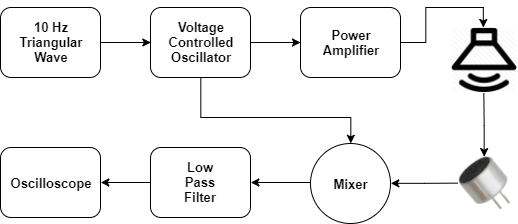
\includegraphics[width=0.47\textwidth]{diagram_Final}
	\caption{\label{fig:diagram_Final}The Overall Block Diagram}
\end{figure}
\section{Transmitter}

\subsection{Voltage Controlled Oscillator}
\begin{figure}[h!]
 \setlength{\unitlength}{\textwidth}
 \center 
 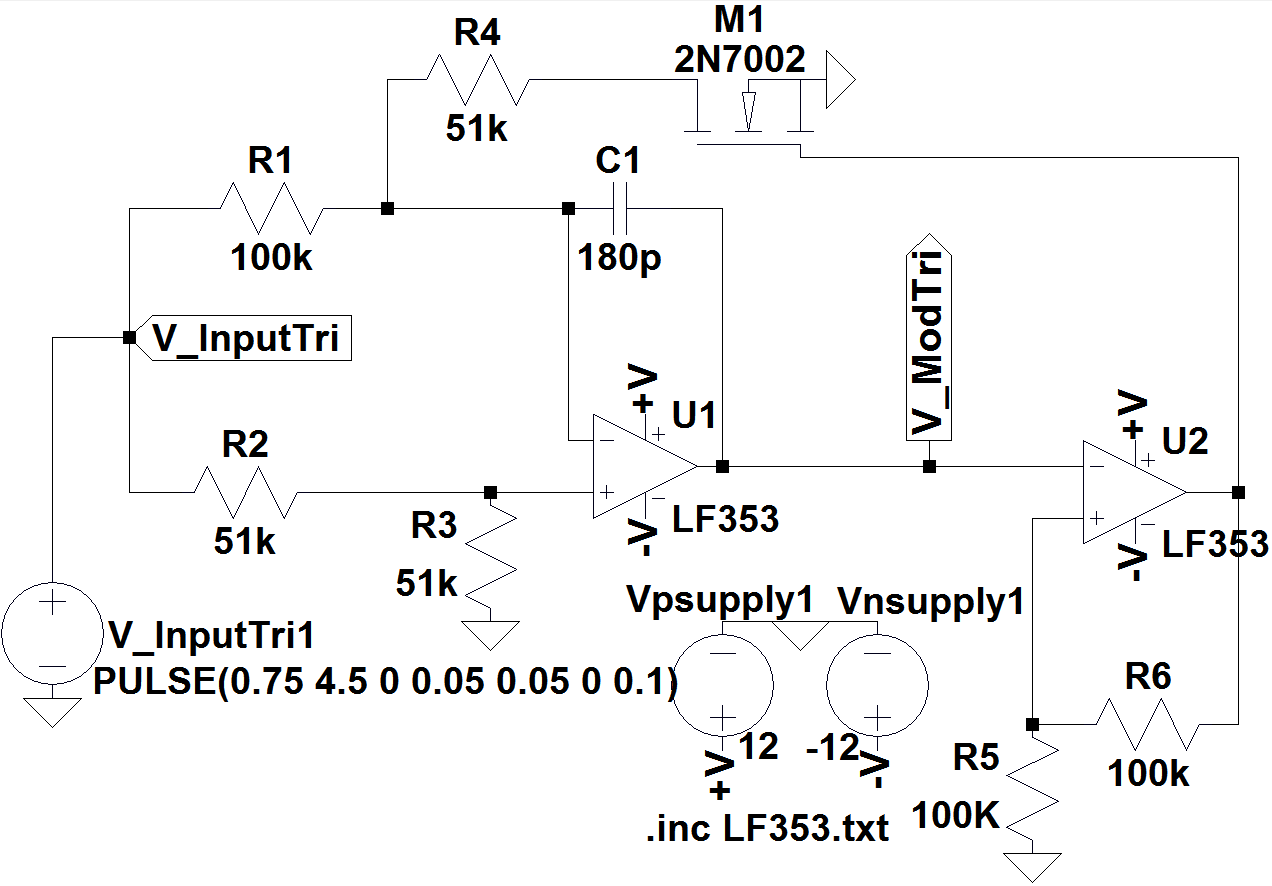
\includegraphics[width=0.45\unitlength]{VCO_Circuit_FinalModified}
 \caption{\label{fig:VCO_Circuit}The Voltage Controlled Oscillator Circuit}
\end{figure}
\begin{figure}[h!]
	\centering
	\begin{subfigure}{.48\textwidth}
		\centering
		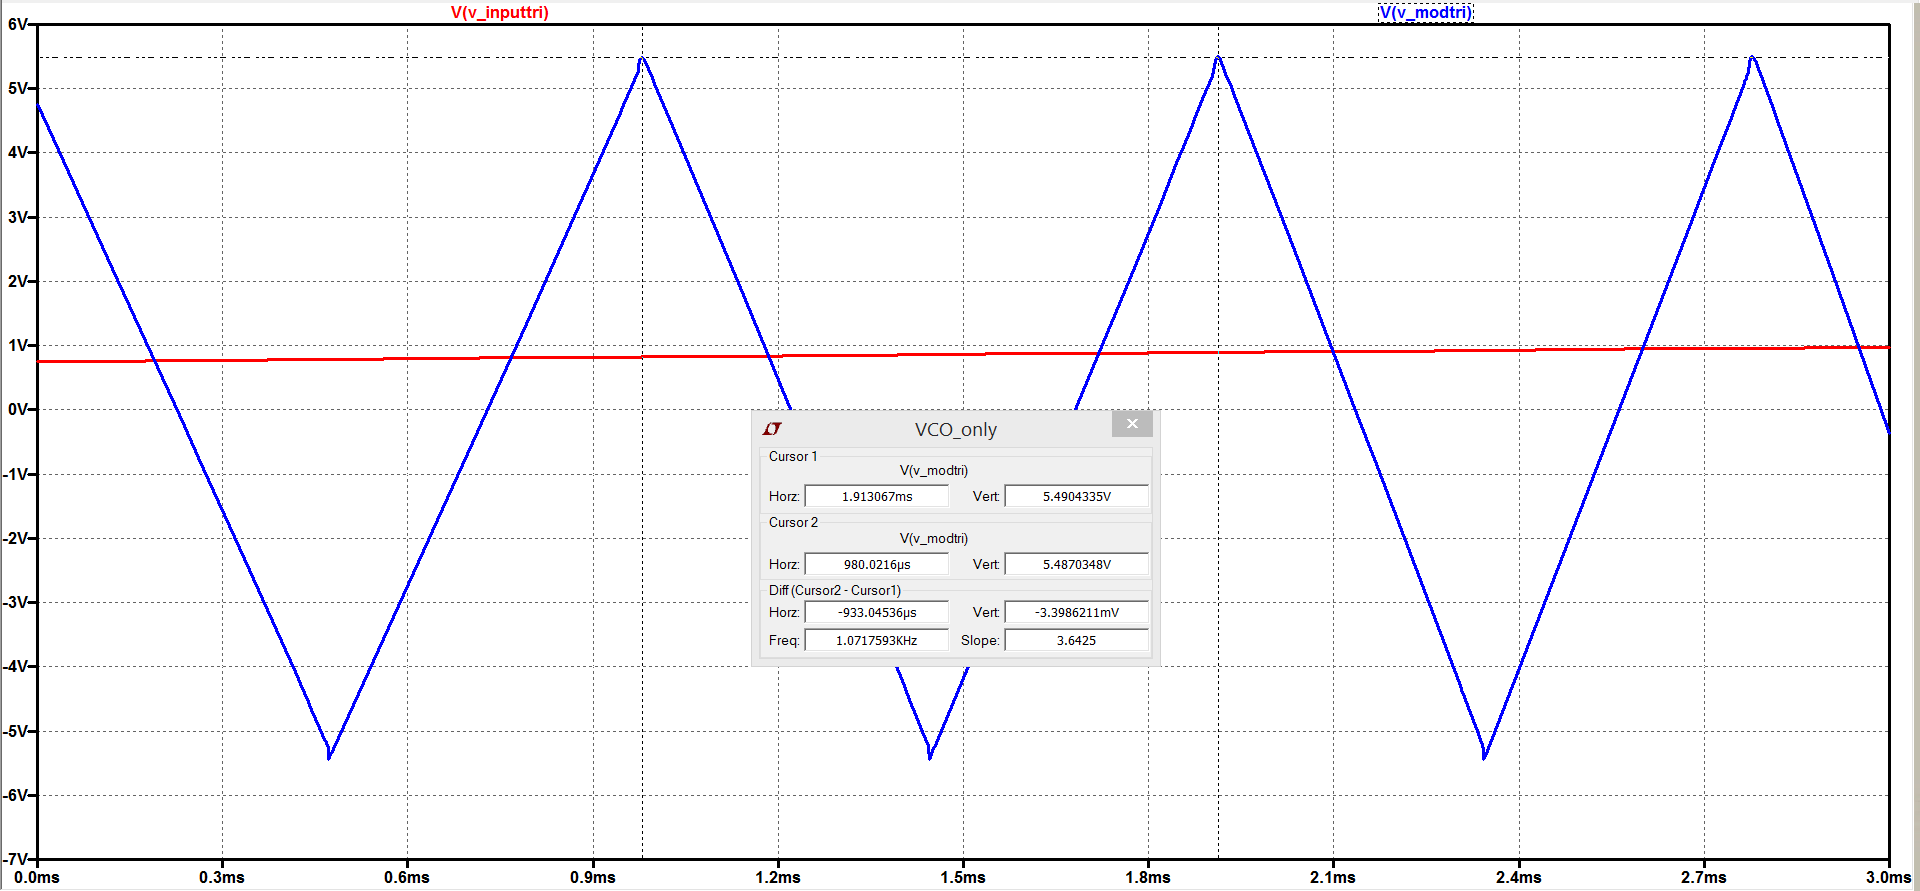
\includegraphics[width=1\linewidth]{scope_28_SimResult}
		\caption{Theoretical Output of VCO.}
		\label{fig:VCOFor1kHzTheoretical}
	\end{subfigure}%
	\newline
	\begin{subfigure}{.48\textwidth}
		\centering
		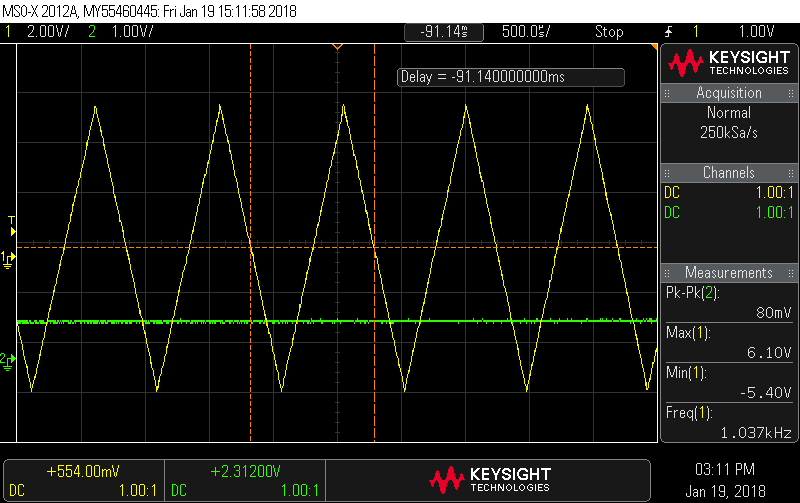
\includegraphics[width=1\linewidth]{scope_28}
		\caption{Practical Output of VCO.}
		\label{fig:VCOFor1kHzPractical}
	\end{subfigure}
	\caption{VCO Outputs for 1kHz.}
	\label{fig:VCOFor1kHz}
\end{figure}

	Voltage controlled oscillator (VCO) is a voltage-to-frequency mapper. VCO outputs variable frequency voltage as the input voltage changes. The used VCO circuit in this project can be seen in \textit{Figure~\ref{fig:VCO_Circuit}}. To be able to generate frequency modulated signal that is the basic function of VCO, the main input to the circuit is a triangular wave. The triangular wave provides varying input voltage so that output frequency changes gradually. The modulated triangular wave is observed at the $V_{ModTri}$ node. Charging and discharging phenomena of capacitor $C_{1}$ is the main reason of the oscillation at the $V_{ModTri}$ node. While capacitor charges, modulated wave climbs down and as capacitor discharges through $R_{4}$, modulated wave climbs up. Capacitor charging-discharging cycles do effect the output frequency, however, are not the real reason of modulated triangular wave at the $V_{ModTri}$ node. If there were a constant DC input, the output would be just an oscillating triangular wave with a certain frequency. The main reason for modulated frequency is the changing input voltage. The output frequency depends on three factors. The first one is the capacitance. As capacitance of $C_{1}$ increases, the ability of holding charge of the capacitor increases. This results in longer cycles meaning lower frequency at the $V_{ModTri}$ node. Secondly, the resistance $R_{1}$ sets a barrier for current flow through $C_{1}$. In other words, as $R_{1}$ increases, the time for $C_{1}$ to charge up becomes longer. Hence longer wave cycles are observed again. Third and last factor is the input voltage value. A higher input voltage implies higher current through $C_{1}$. Thus, the time for $C_{1}$ to charge up becomes shorter. As a result, higher frequencied cycles are observed at the $V_{ModTri}$ node.

\begin{figure}[t!]
	\centering
	\begin{subfigure}{.48\textwidth}
		\centering
		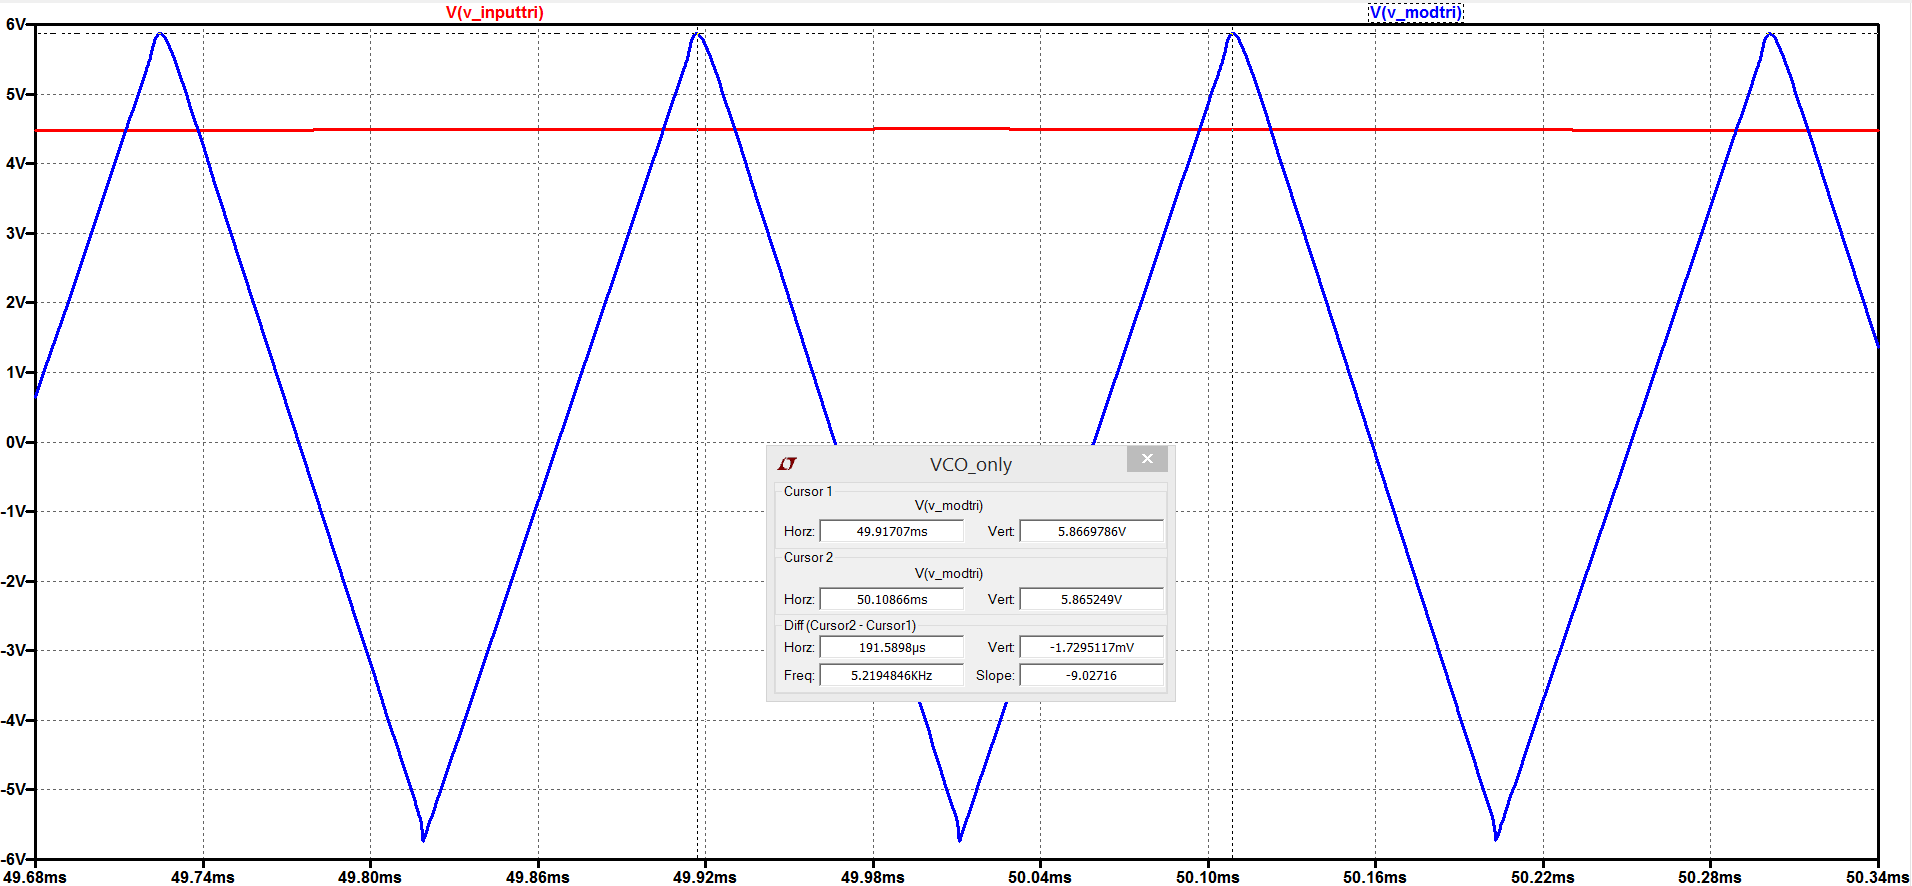
\includegraphics[width=1\linewidth]{scope_24_SimResult}
		\caption{Theoretical Output of VCO.}
		\label{fig:VCOFor5kHzTheoretical}
	\end{subfigure}%
	\newline
	\begin{subfigure}{.48\textwidth}
		\centering
		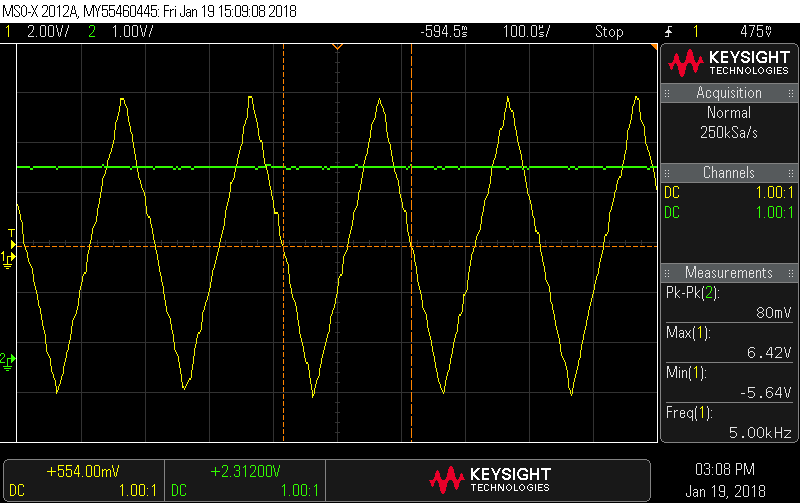
\includegraphics[width=1\linewidth]{scope_24}
		\caption{Practical Output of VCO.}
		\label{fig:VCOFor5kHzPractical}
	\end{subfigure}
	\caption{VCO Outputs for 5kHz.}
	\label{fig:VCOFor5kHz}
\end{figure}
To handle these frequent voltage changes, high slew rated LF353\cite{b2} opamps are used. Also for biasing purposes, a N-MOS with low open voltage provides lower DC offset at the input $V_{InputTri}$. 2N7000\cite{b3} model N-MOS suits for this application. Simulation and theoretical results for two corner frequencies are presented in \textit{Figure~\ref{fig:VCOFor1kHz}} and \textit{Figure~\ref{fig:VCOFor5kHz}}. VCO outputs are revealed as expected in theoretical results. The resistor and capacitor values are chosen initially by observing examples on websites\cite{b4} and later by trial and error. The ratio of $\frac{R_{5}}{R_{5}+R_{6}}$, which is the threshold voltage of the Schmitt Trigger represented with $U_{2}$, sets the peak voltage of the $V_{ModTri}$. This voltage is $\sim6V$ in our design.
\subsection{Power Amplifier and Speaker}
\begin{figure}[t!]
 \setlength{\unitlength}{\textwidth}
 \center 
 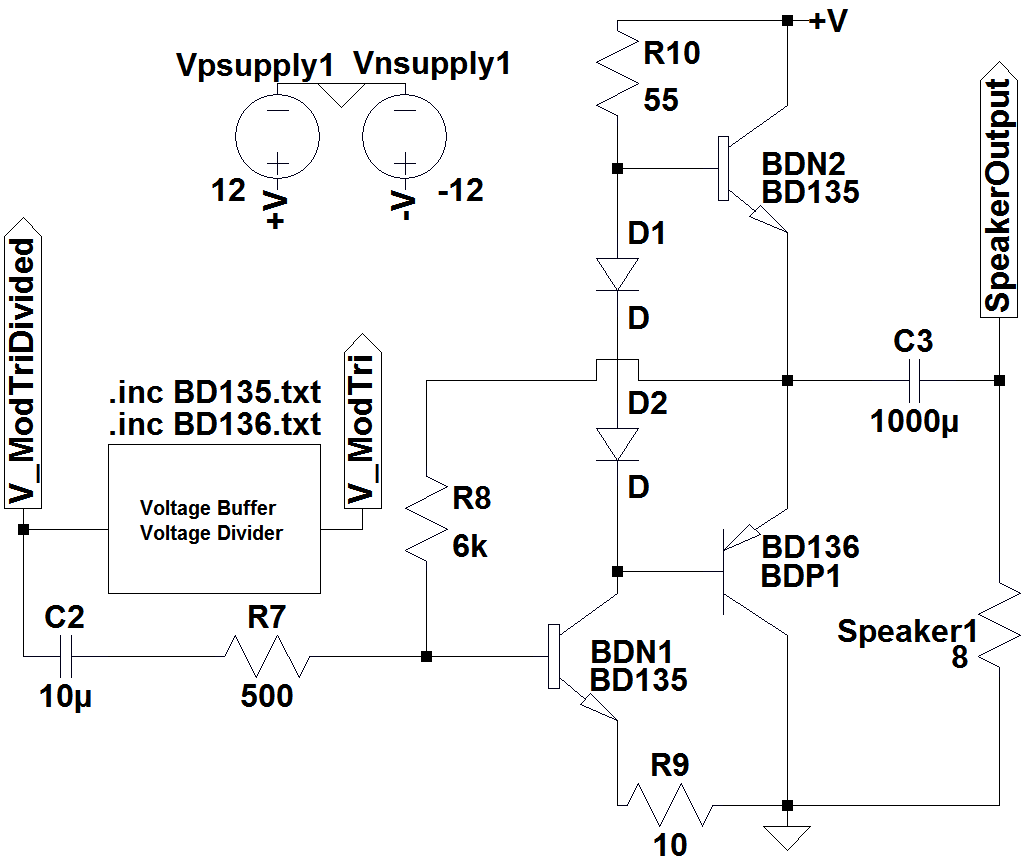
\includegraphics[width=0.45\unitlength]{PowerAmp_Circuit_FinalModified}
 \caption{\label{fig:PowerAmp_Circuit}Power Amplifier Circuit Driving the Speaker}
\end{figure}
This part is aimed to transmit the frequency modulated signal, which is the output of the VCO, to a medium by using a power amplifier. A Class AB amplifier is utilized for this purpose. The amplifier is basically composed of two stages that are common emitter driver and AB amplifier.

The main transistor of common emitter driver is $BDN_{1}$. This transistor sets the DC biasing of $BDN_{2}$ and $BDP_{1}$. It may be considered as a current source. Also, the input signal is output as inversely polarized at the collector of the $BDN_{1}$.

The class AB amplifier mainly consists of two transistors one of which is a NPN and the other is PNP. The diodes $D_{1}$ and $D_{2}$ are to provide Q point stability of the transistors. Also they provide constant voltage difference between the bases of $BDN_{2}$ and $BDP_{1}$. When the voltage in positive cycle, $BDN_{2}$ amplifies the signal whereas $BDP_{1}$ amplifies the signal in negative cycle. These transistors operate cooperatively according to the cycle of the signal. Lastly, feedback resistor $R_{1}$ reduces the distortion of the output signal by introducing a negative feedback to the input signal in shunt-shunt topology. On the other hand, the DC biasing of $BDN_{1}$ is improved with the use of $R_{1}$.

The simulation results for power amplifier regarding current through and voltage across speaker is shown in \textit{Figure~\ref{fig:PowerAmp_speakerOutput}}. The rms of triangular wave can be found by $\frac{V_{peak}}{\sqrt{3}}$. With this in mind, power consumed by the speaker is simply $\frac{4.3V\times0.53A}{3}\approx0.76$ Watts. In breadboard, however, the circuit didn't function properly. In simulation, transistors were all in forward active region and $BDN_{2}$ and $BDP_{1}$ were satisfying $12V-6V-0V$ DC voltage biasing as in \textit{Figure~\ref{fig:PowerAmp_Circuit_dcParameters}}.
\begin{figure}[t!]
	\setlength{\unitlength}{\textwidth}
	\center 
	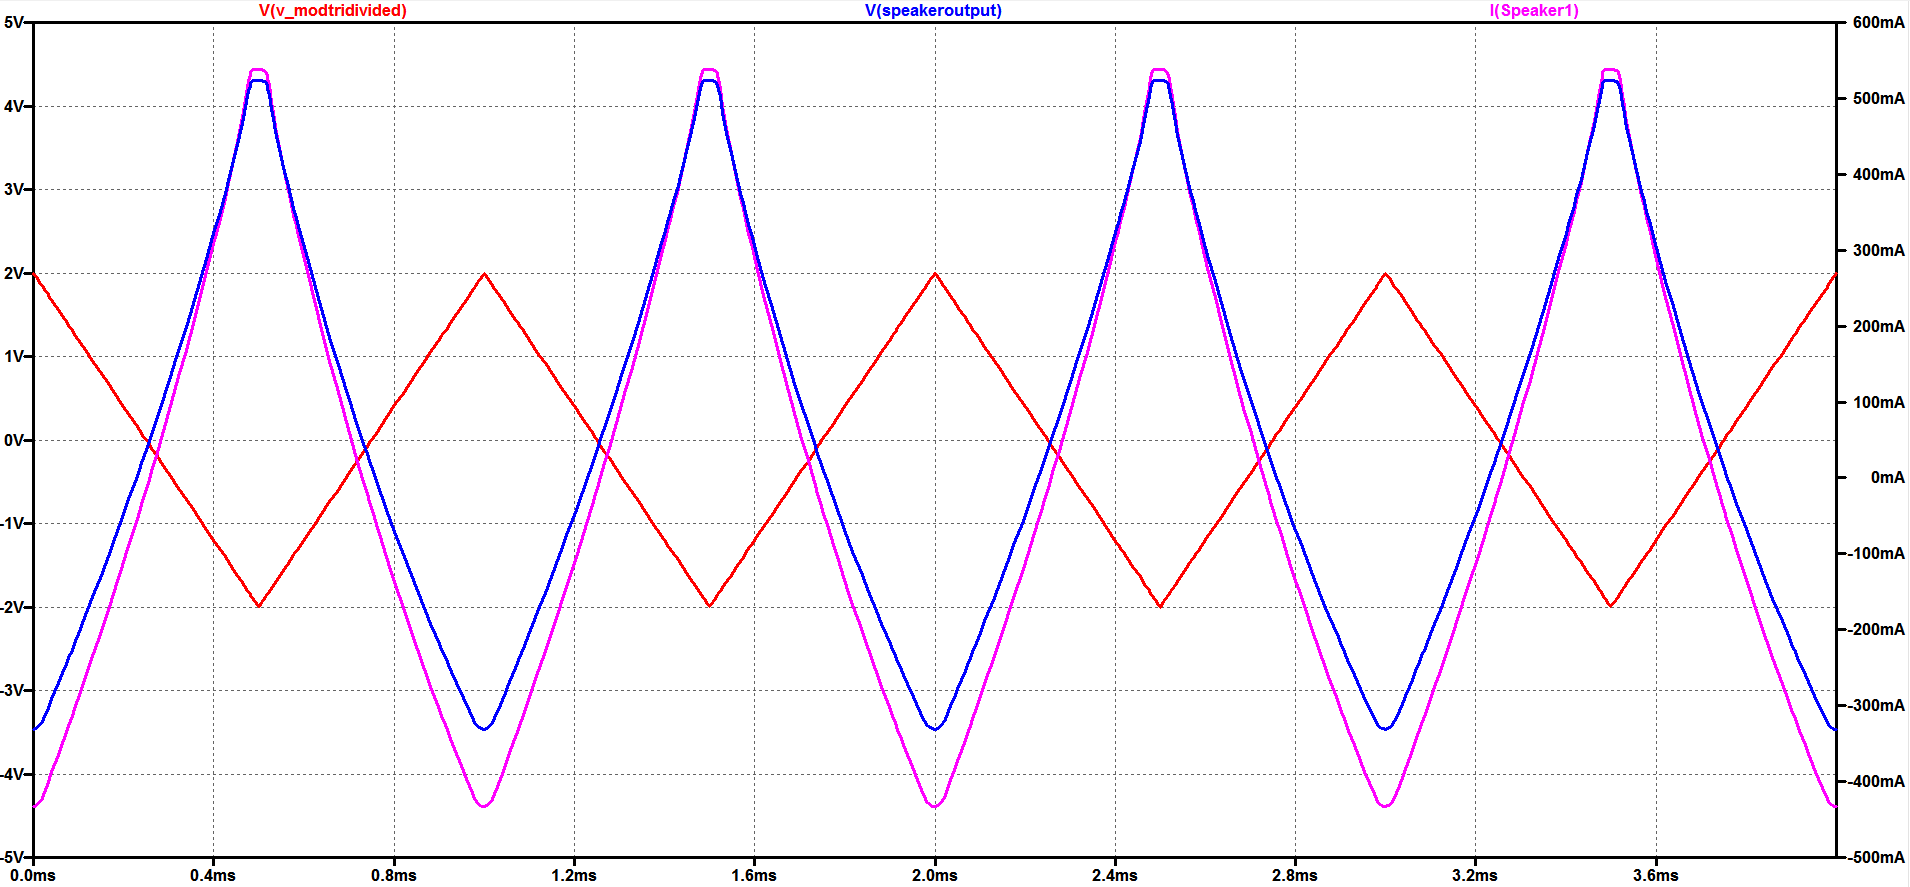
\includegraphics[width=0.48\unitlength]{PowerAmp_speakerOutput}
	\caption{\label{fig:PowerAmp_speakerOutput}Power Amplifier Voltage Waveforms Across Speaker}
\end{figure}
\begin{figure}[t!]
	\setlength{\unitlength}{\textwidth}
	\center 
	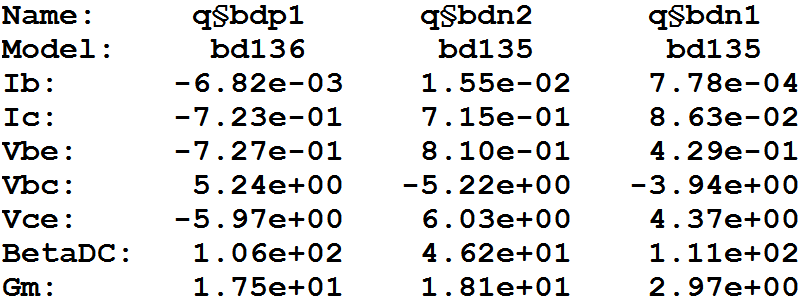
\includegraphics[width=0.45\unitlength]{PowerAmp_Circuit_dcParameters}
	\caption{\label{fig:PowerAmp_Circuit_dcParameters}Power Amplifier Circuit DC Biasing Parameters}
\end{figure}

\section{Receiver}

\subsection{Microphone \& Microphone Driver}
	To receive the sound signal coming from the speaker and turn it into a electrical signal, some kind of speaker should be used. For this purpose, an electret microphone will be used. 
	
	To drive the electret microphone, a driver circuit is designed. The design should include feeding for the transistor inside the microphone and amplify the output signal since the output signal would be too small to be used. But before amplifying the signal, we shall remove possible dc offsets and noises by a passive high pass filter. The designed driver can be seen at \textit{Figure~\ref{fig:micdr}}.

\begin{figure}[h!]
\setlength{\unitlength}{\textwidth}
\center 
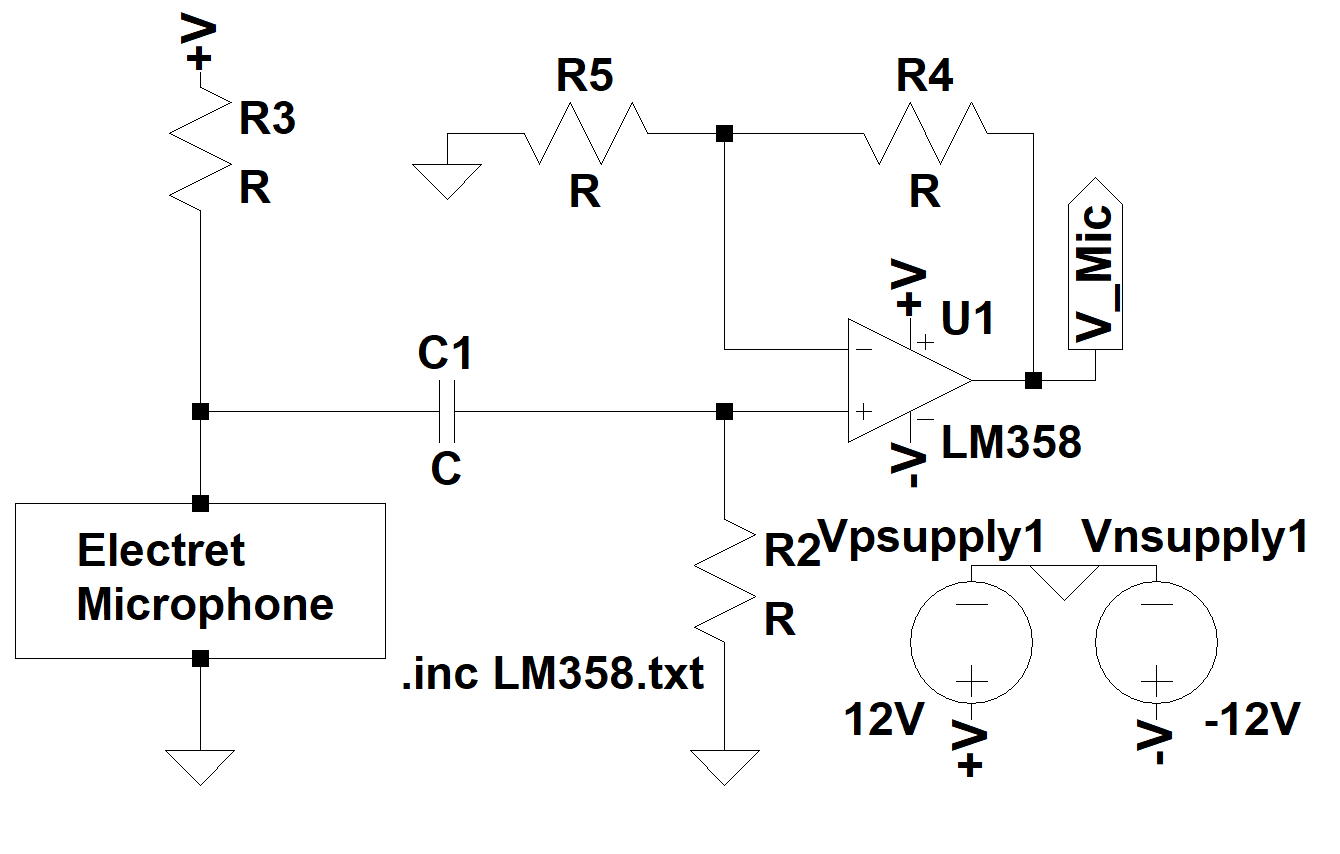
\includegraphics[width=0.45\unitlength]{mic_v2.png}
\caption{\label{fig:micdr}Driver Circuit for Electret Microphone }
\end{figure}	


By node analysis, the lower cutoff frequency of the highpass filter can be found as

%\begin{equation}
$$ f_{c} =\frac{1}{2\pi R_{2}C_{1}} $$
%\end{equation}

If we take $R_{2}=10k\Omega$ and $C_{1}=0.1\mu F$, cutoff frequency $f_c$ can be found as

%\begin{equation}
$$ f_{c} =\frac{1}{2\pi*10~k\Omega*0.1~\mu F}\approx 159 Hz $$
%\end{equation}

The resulting $f_c$ will be enough to remove noise and DC offsets.

\begin{figure}[h!]
\setlength{\unitlength}{\textwidth}
\center 
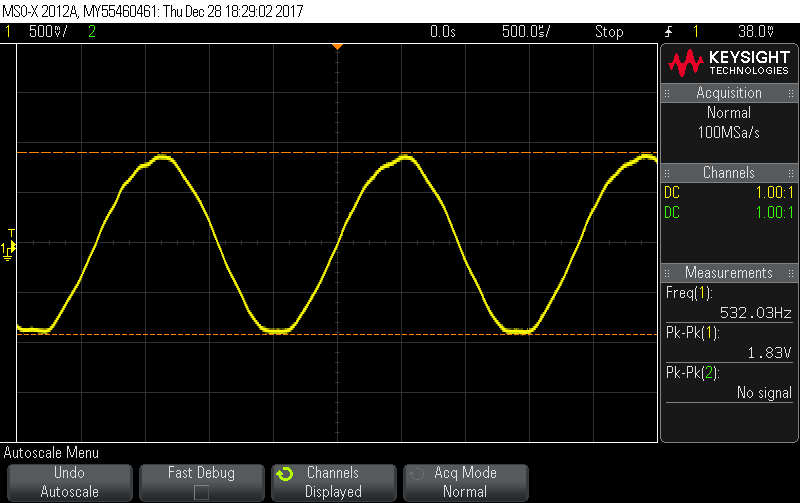
\includegraphics[width=0.45\unitlength]{mic_osc.png}
\caption{\label{fig:micout} Output Signal of Microphone Circuit at Laboratory }
\end{figure}	

	The Output waveform for the microphone circuit for given sound signal at the laboratory can be seen at \textit{Figure~\ref{fig:micout}}.


%\subsection{Automatic Gain Controller}
%	Automatic gain controller is a circuit that controls gain and adjusts the amplitude of the output signal automatically. Since the output of the microphone depends on distance and frequency, AGC should be used to adjust the amplitude of the output  signal of microphone driver circuit. For that purpose a circuit at the \textit{Figure~\ref{fig:agc}} for automatic gain control in Wien Bridge will be used.

%\begin{figure}[h!]
%\setlength{\unitlength}{\textwidth}
%\center 
%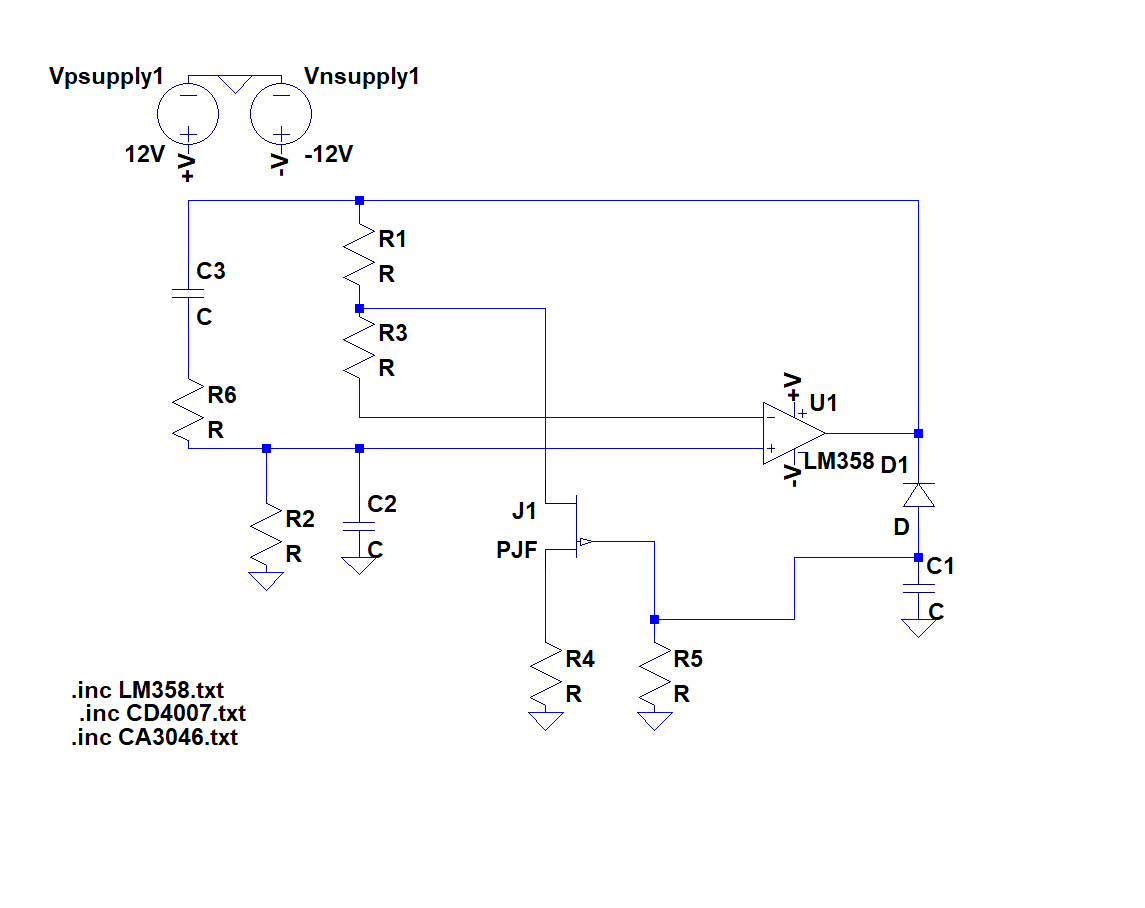
\includegraphics[width=0.5\unitlength]{agc.png}
%\caption{\label{fig:agc} Automatic Gain Control in Wien Bridge }
%\end{figure}	

	
	
\subsection{Mixer}
	
	Mixer is the device that accepts two input signals and gives a output signal that consists of two distinct signals with different frequencies. While, one of these signals has a frequency that is equal to the difference between the frequencies of first signal and second signal, other signal has a frequency that is summation of the frequencies of first and second signal. In other words, if we assume input signal 1 has a frequency $f_1$ and input signal 2 has a frequency $f_2$. The output signal would look like  
	
	$$ O/P~~ Signal ~=~ A(f_1+f_2) + B(|~f_1 -f_2~|)  $$
	
	where A and B are the signals having frequencies  
	
	$$	f_A ~= ~ f_1+f_2~~ \&$$
	$$	f_B~=~|~f_1 -f_2~| $$ 
	
	respectively. 
	
	
\begin{figure}[h!]
\setlength{\unitlength}{\textwidth}
\center 
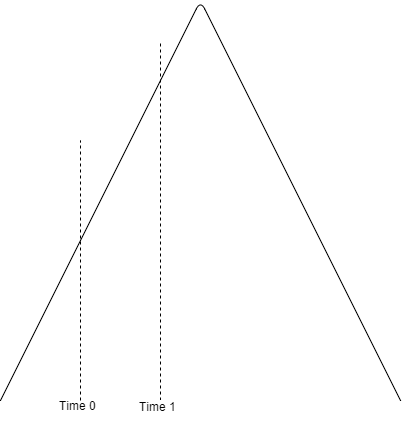
\includegraphics[width=0.25\unitlength]{triangular.png}
\caption{\label{fig:trimix}One Period of Triangular Wave }
\end{figure}		
	
	We also know that the distance between source and receiver causes a time delay proportional to the distance for the received signal in comparison to the transmitted signal. Thanks to triangular wave and the voltage controlled oscillator we used at the beginning of the project, the distance between the source and receiver is also proportional to the the frequency difference between original source signal and received signal by receiver. This can be understood from the basic principle of VCO. Assume that the first signal left the VCO and entered the mixer at Time 0 and has a frequency $f_1$ proportional to the magnitude of triangular wave at Time 0. Similarly second signal entered the Mixer at Time 1 and has a frequency $f_2$ proportional to the magnitude of triangular wave at Time 1. One period of the input triangular wave and "Time 0" \& "Time 1" on top of it can be seen at \textit{Figure~\ref{fig:trimix}}. 
	
	Therefore, the time shift "$~Time~1-Time~0~$" is proportional to the "$|~f_2-f_1~|$". Thus, if we can find the frequency difference between this signal, we can easily find the desired distance since the distance can be found by
	$$ d~=~(Time~1-Time~0)*v_s~=~K*|~f_1-f_2~|$$ 
	where K is a constant and $v_s$ is the speed of sound.
	
	
\begin{figure}[h!]
\setlength{\unitlength}{\textwidth}
\center 
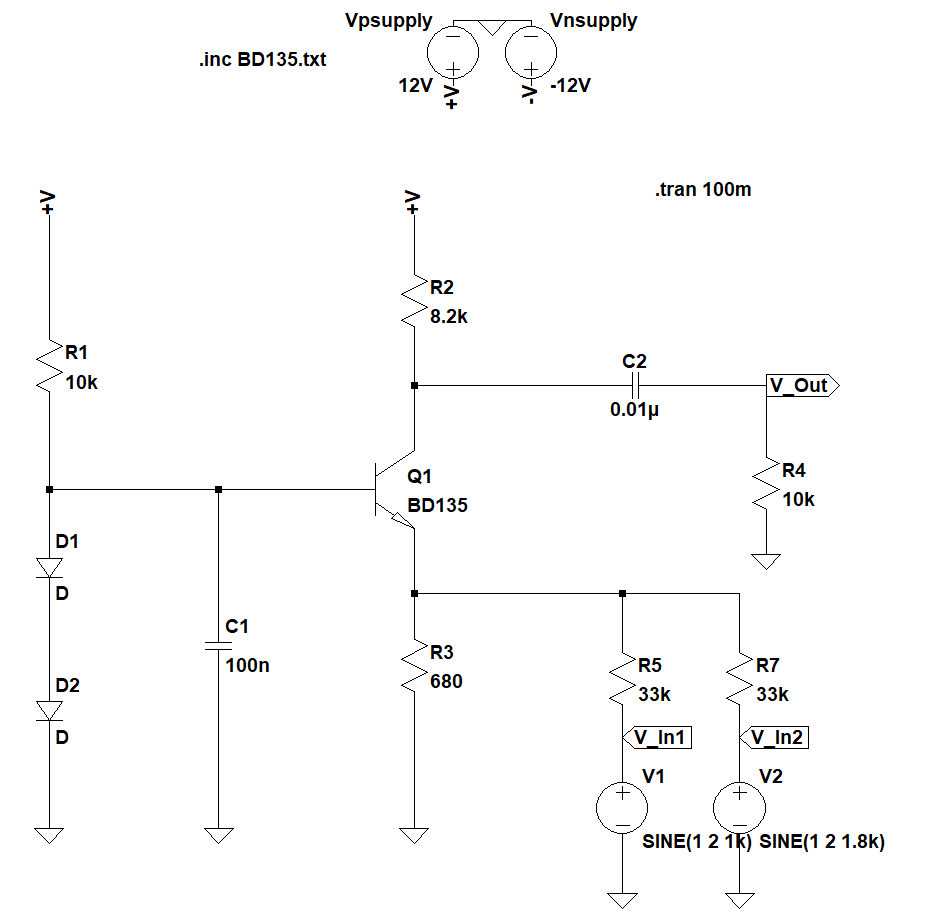
\includegraphics[width=0.45\unitlength]{mixer_v2_2.png}
\caption{\label{fig:mixer}A Mixer Circuit }
\end{figure}	


	The value of the constant $'K'$ can be found easily by considering the time that takes for the voltage controlled oscillator to span the half of the rectangular wave. In other words, the wave spans the 4 kHz frequency distance at half period, that is $\frac{1}{20}~second~$ for 10 Hz. Therefore, for any frequency difference to happen, the time takes can be found to be as
	$$	t~=~\frac{f*T}{2}*\frac{1}{4~k}~=~\frac{f}{80}*10^{-3}~second	$$
	Thus, the distance between source and receiver can be by considering the time takes for any frequency difference and the distance sound wave can cover at that frequency, that is 
	$$	d~=~v_s~*~t~=~\frac{v_s*f}{80}*10^{-3}~=\frac{343*f}{80}*10^{-3}~meter	$$    	
	$$	d~=~4.2875*f*10^{-3}~meter	$$	
	
	\-\\	
	Thus, the constant $'K'$ can be found as
	$$	K~=~4.2875*10^{-3}~meter	$$	
	and the distance measured can be found as 
	$$	d_{measured}~=~K*f_B~=~4.2875*f_B*10^{-3}~meter	$$	
	where $f$ and $f_B$ are the unitless numerical values of the frequency difference.
	
	
	For that reasons, a mixer circuit is a very crucial part of our project to be designed. A basic mixer circuit we have used can be seen at \textit{Figure~\ref{fig:mixer}}.


\begin{figure}[h!]
\setlength{\unitlength}{\textwidth}
\center 
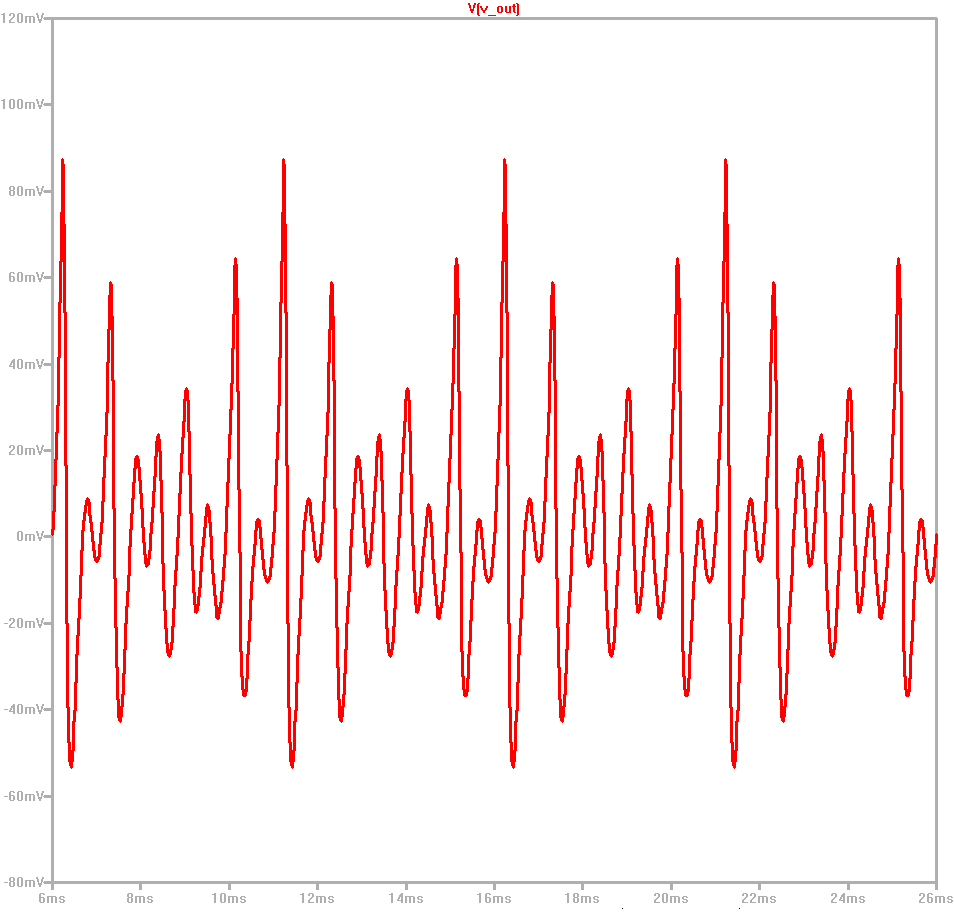
\includegraphics[width=0.45\unitlength]{mixer_op3.png}
\caption{\label{fig:mixerop} The Output Waveform of the Mixer Circuit }
\end{figure}	

	
	To test our design, we have used LTSpice for simulations. Applying two sinusoidal inputs from $33k\Omega$ resistor with $1~kHz$ frequency \& $1.8~kHz$ frequency, we observed the output waveform at the \textit{Figure~\ref{fig:mixerop}}. To understand whether it works or not, the 'FFT Spectrum Analysis' was used. As can be seen from the \textit{Figure~\ref{fig:mixerfft}}, we have observed impulses at input frequencies, at difference frequency , at total frequency and their second and higher harmonics. Since we would use low-pass filter after the mixer, we were not worried about the higher order harmonic since they would be eliminated at the output anyway. 

	To test the design at the laboratory, we have used similar methods. By using two signal generators, we supplied the mixer circuit with two sinusoidal signal with different frequencies. The output waveform after that procedure can be seen at \textit{Figure~\ref{fig:mixerosc1}}.
	
	After finding the proper mixer circuit, the only step-back from measuring the measuring the distance was designing a proper low pass filter. Since we wanted the filter to have sharp frequency response we have used second order low pass filter. The following section will explain the design steps of the filter.   


\begin{figure}[h!]
\setlength{\unitlength}{\textwidth}
\center 
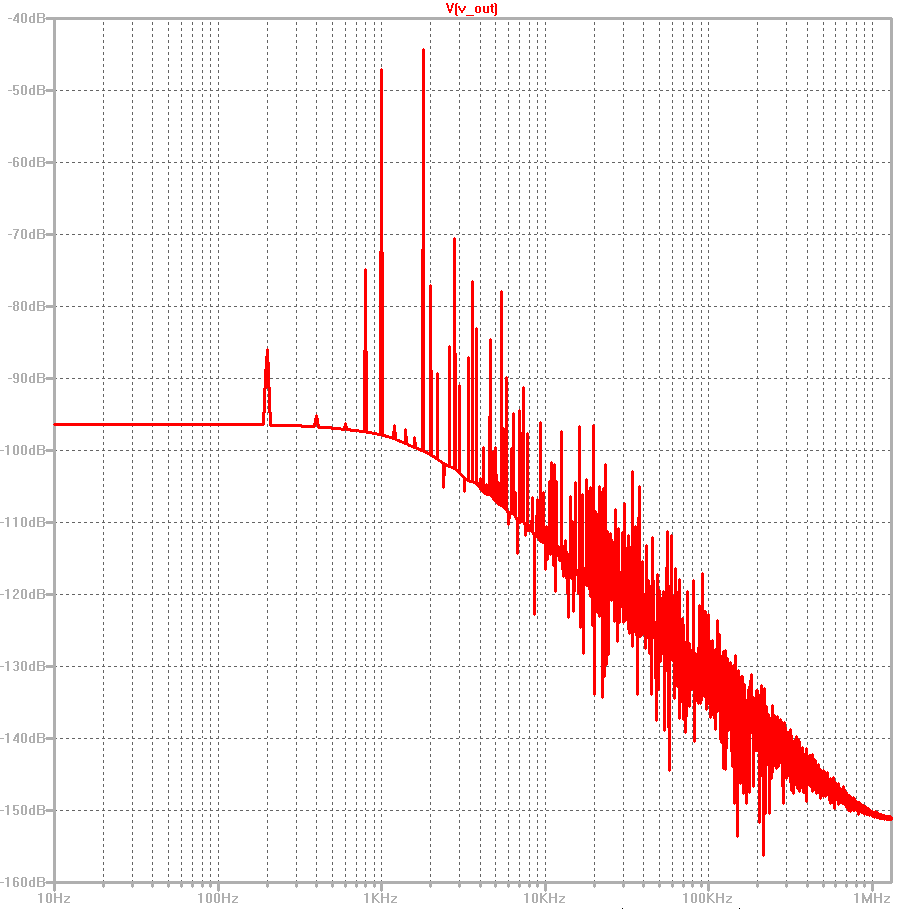
\includegraphics[width=0.45\unitlength]{mixer_fft3.png}
\caption{\label{fig:mixerfft} The Output FFT Waveform of the Mixer Circuit }
\end{figure}	


\begin{figure}[h!]
\setlength{\unitlength}{\textwidth}
\center 
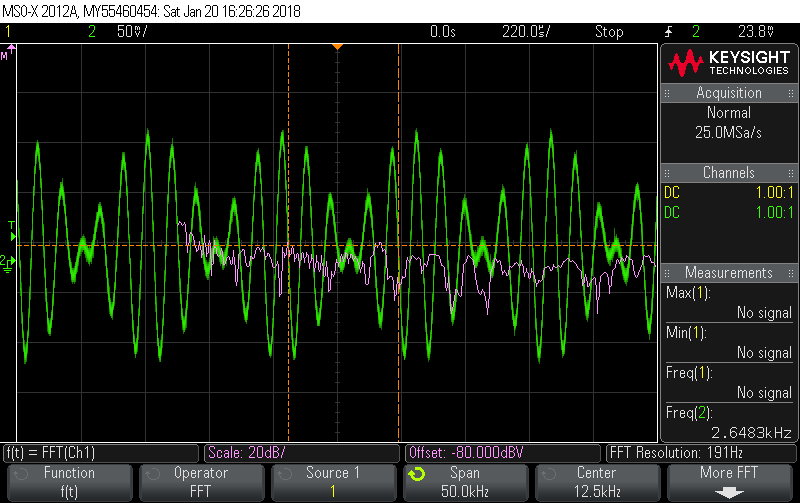
\includegraphics[width=0.45\unitlength]{mixer_osc1.png}
\caption{\label{fig:mixerosc1} The Practical Output Waveform of the Mixer Circuit }
\end{figure}	


%\begin{figure}[h!]
%\setlength{\unitlength}{\textwidth}
%\center 
%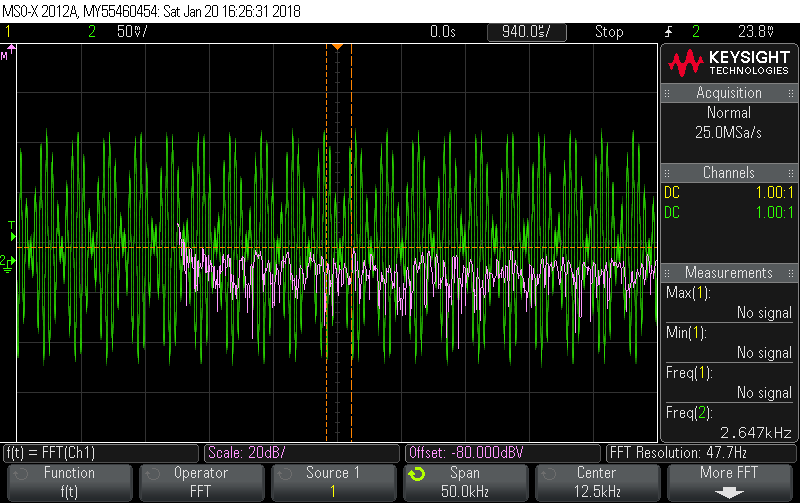
\includegraphics[width=0.45\unitlength]{mixer_osc2.png}
%\caption{\label{fig:mixerosc2} The Practical Output Waveform of the Mixer Circuit }
%\end{figure}	

		
				
\subsection{Low Pass Filter}


	Unfortunately, the output signal of the Mixer did not only carry the frequency difference information but also frequency summation information. Since we are only interested in the difference between the frequencies only, a low pass filter was used to extract the wanted signal.


\begin{figure}[h!]
	\setlength{\unitlength}{\textwidth}
	\center 
	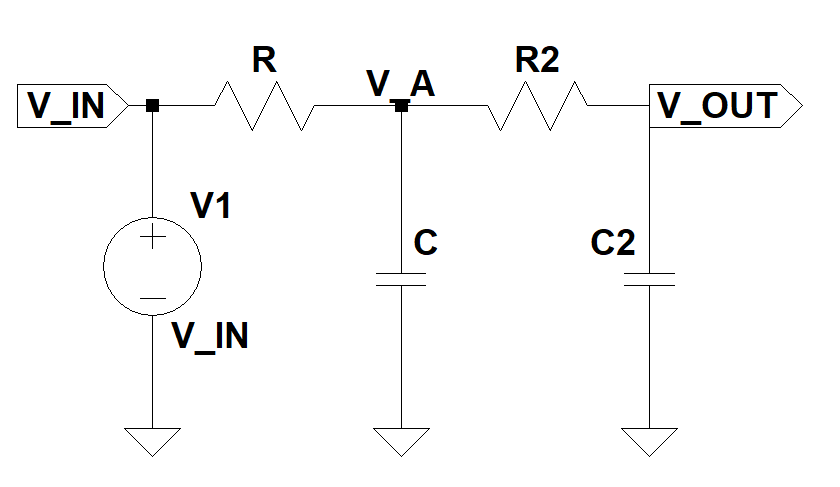
\includegraphics[width=0.5\unitlength]{lpf_v4.png}
	\caption{\label{fig:pslpf}A Passive Second Order Low-Pass Filter }
\end{figure} 	
	
	Low Pass Filters are the type of filters that passes the signals having the frequencies lower that the desired frequencies also known as the cut-off frequencies of the filter. Other signals having higher frequencies would be eliminated at the output of the low pass filter. Low pass filter can be categorized by their included capacitor number. For instance, if one low pass filter includes only one capacitor and resistor, it can be named as first order low pass filter. Similarly, a filter with two capacitor can be considered as second order low pass filter. In our design we preferred to use a second order low pass filter in order to get sharp enough frequency response. A basic second order low-pass filter can be seen at \textit{Figure~\ref{fig:pslpf}} \\ 
	
	Low pass filters can also be categorized into two main type that are active filters and passive filters. Active filters are the ones that can amplify the desired signals and eliminate otherwise. These type of filters generally includes an op-amp for that purpose.  A simple active second order low-pass filter can be seen at \textit{Figure~\ref{fig:lpf}}. Whereas the passive low pass filters can only supply desired output signal with maximum unity gain. A general passive second order low-pass filter can be seen at \textit{Figure~\ref{fig:pslpf}}.  		 

	After considering the active one, we have decided using a passive second order low pass filter at \textit{Figure~\ref{fig:pslpf}}. For choosing proper resistance and capacitance values, the some KCL and KVL operations can be conducted on the circuit at S-Domain.
	
	$$	V_A~=~\frac{V_{in}*R}{R+\frac{1}{sC}//(R_2+\frac{1}{sC_2})}	$$  	
	
	$$	V_{out}~=~\frac{V_A*\frac{1}{sC_2}}{R_2+\frac{1}{sC_2}}	$$	

	Transfer function being	
	
	$$ H(s)~=~\frac{V_{out}}{V_{in}}$$
	
	Cut-off frequency can be found by rearranging terms into wanted form. If we equate $R~=~R_1$ \& $C~=~C_1$ for the simplicity, after some effort the cut-off frequency can be found as
	
	$$	f_c ~=~ \frac{1}{2\pi RC}	$$
	
	The resistance values can be found from there by assuming the capacitor values for desired frequency. For 
	
	$$~f~=~1.5~kHz~=~1.5*10^3~Hz $$ 
	$$ \& $$ 
	$$~C~=~10~nF~=~10^{-8}~F$$
	Resistance $R$ can be found as
	$$ R~=\frac{1}{2\pi*1.5*10^3*10^{-8}}\approx~10~k\Omega $$
	
	


\begin{figure}[h!]
	\setlength{\unitlength}{\textwidth}
	\center 
	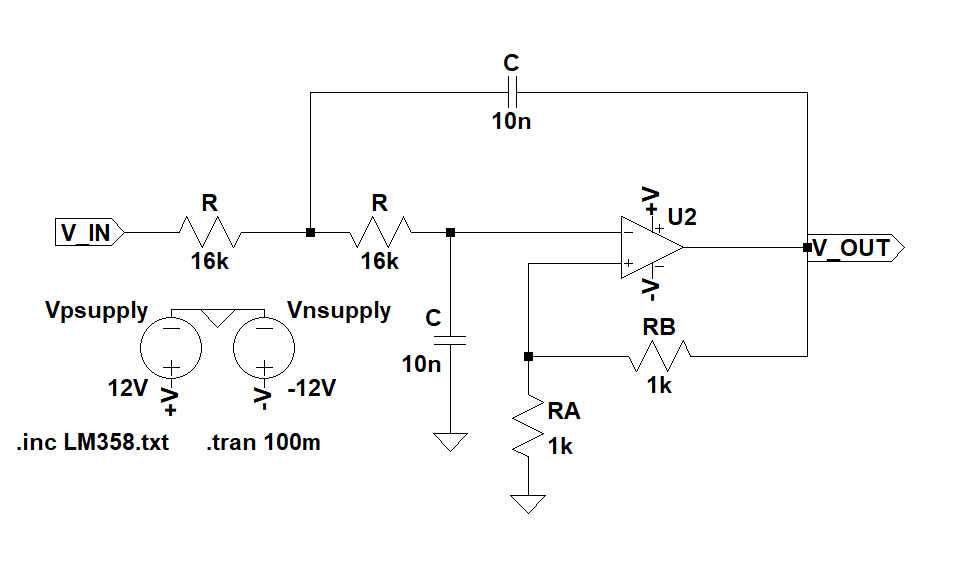
\includegraphics[width=0.5\unitlength]{lpf_v2.png}
	\caption{\label{fig:lpf}An Active Second Order Low-Pass Filter }
\end{figure} 
	
	\-\\ \-\\ \-\- To test the filter at dasjbdjasdjasvdjhavsdjgasvdjgasvdjgawvjgdjgadjaewjd 
	
	
\begin{figure}[H]
	\setlength{\unitlength}{\textwidth}
	\center 
	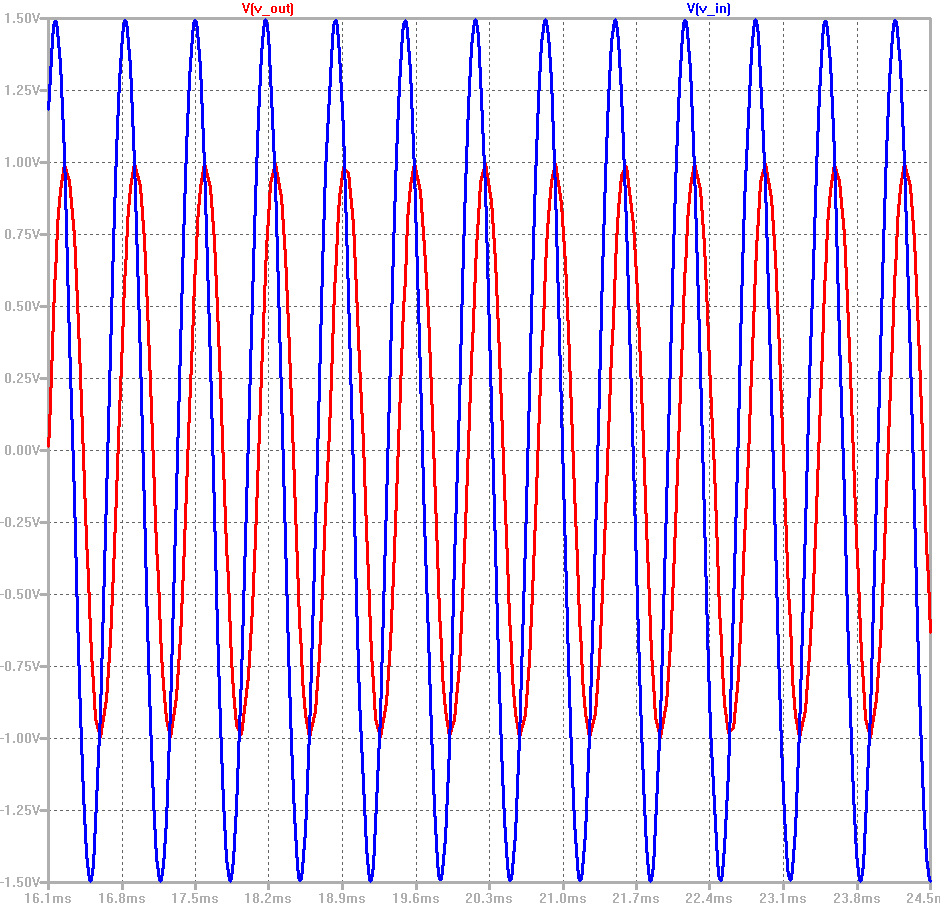
\includegraphics[width=0.45\unitlength]{lpf_op3.png}
	\caption{\label{fig:lpfop3}The Input \& Output Signals for 1.5 kHz}
\end{figure} 


\begin{figure}[H]
	\setlength{\unitlength}{\textwidth}
	\center 
	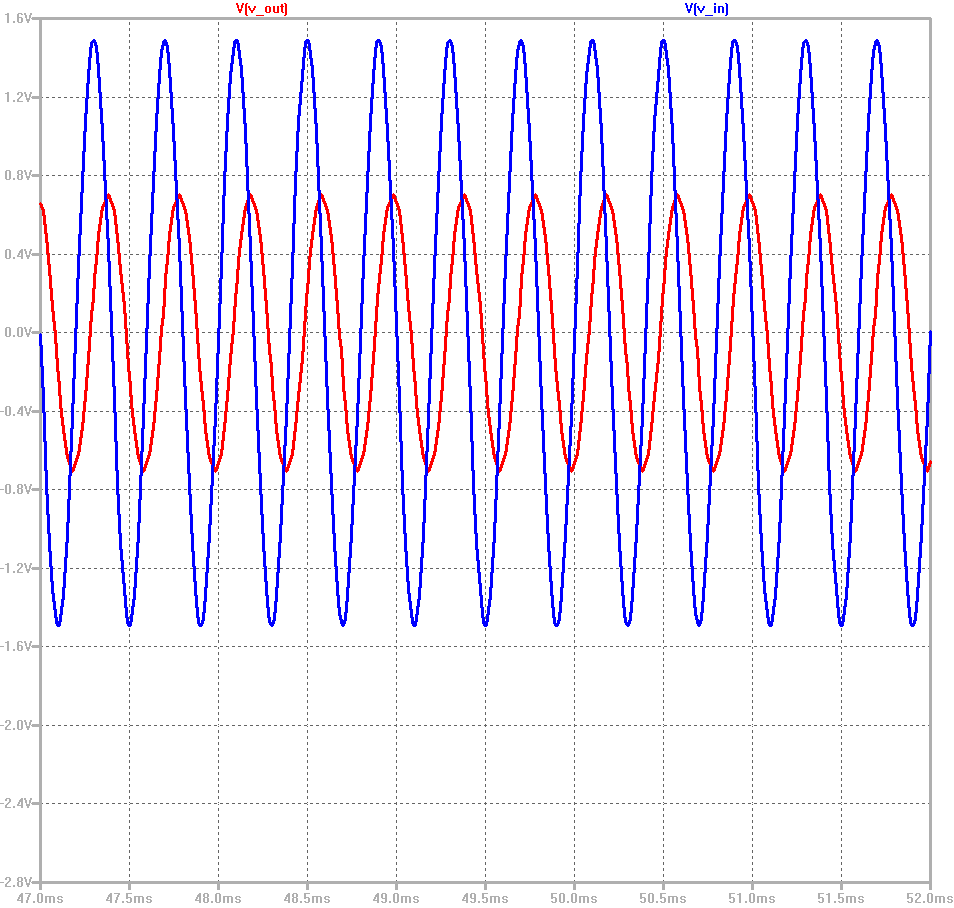
\includegraphics[width=0.45\unitlength]{lpf_op4.png}
	\caption{\label{fig:lpfop4}The Input \& Output Signals for 2.5 kHz}
\end{figure} 


\begin{figure}[H]
	\setlength{\unitlength}{\textwidth}
	\center 
	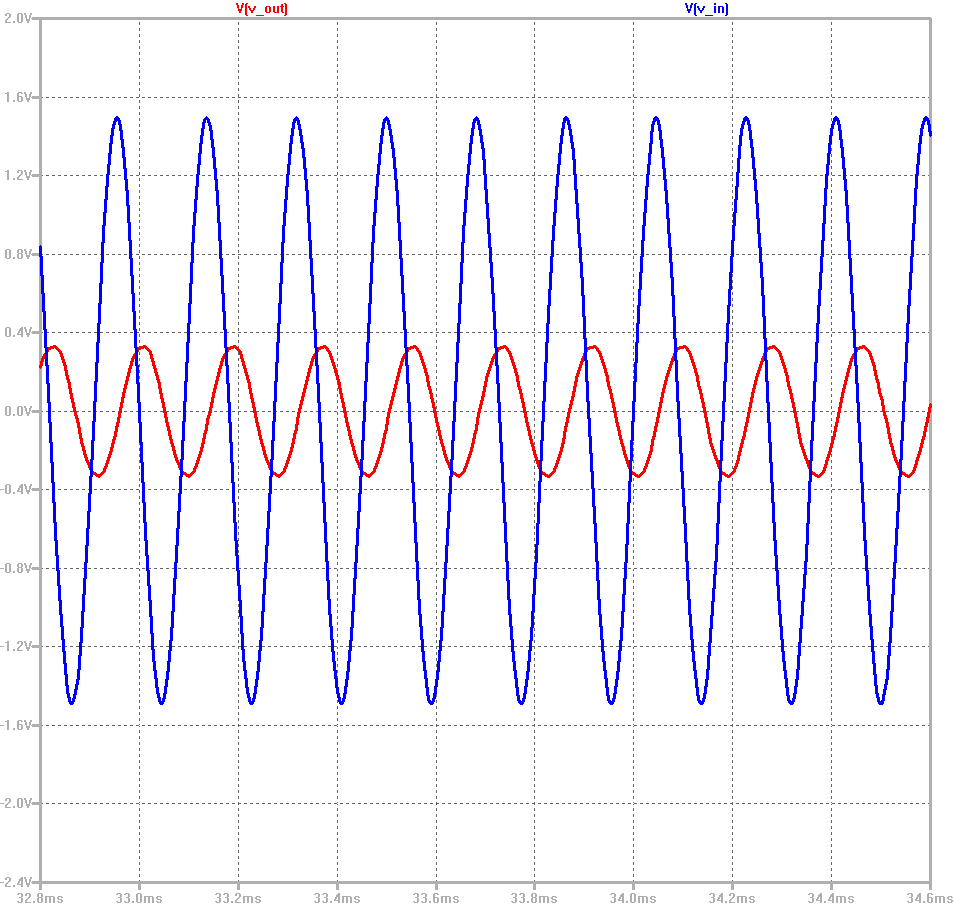
\includegraphics[width=0.45\unitlength]{lpf_op5.png}
	\caption{\label{fig:lpfop5}The Input \& Output Signals for 5 kHz}
\end{figure} 


	

\begin{figure}[H]
	\setlength{\unitlength}{\textwidth}
	\center 
	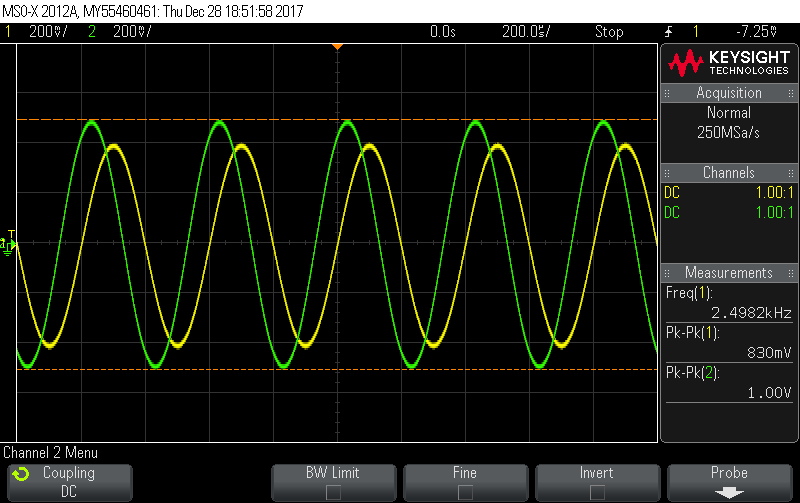
\includegraphics[width=0.45\unitlength]{lpf_osc4.png}
	\caption{\label{fig:lpfosc4}Practical Output Signal for 2.5 kHz}
\end{figure} 
	

\begin{figure}[H]
	\setlength{\unitlength}{\textwidth}
	\center 
	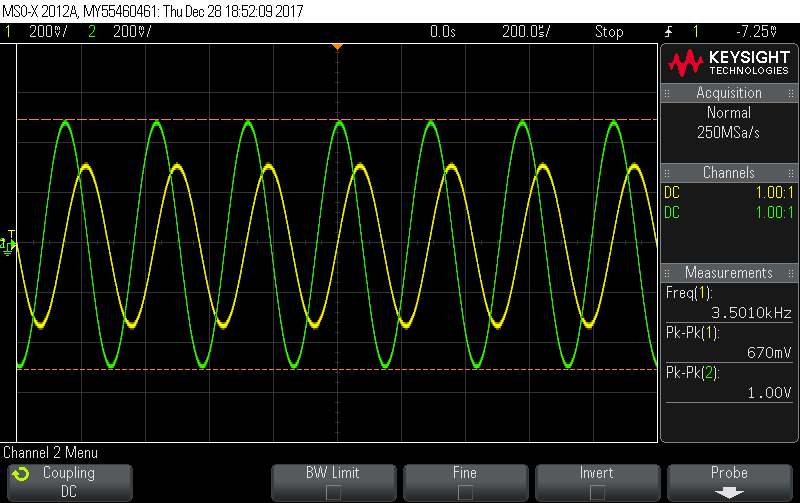
\includegraphics[width=0.45\unitlength]{lpf_osc5.png}
	\caption{\label{fig:lpfosc5}Practical Output Signal for 3.5 kHz}
\end{figure} 
		

\begin{figure}[H]
	\setlength{\unitlength}{\textwidth}
	\center 
	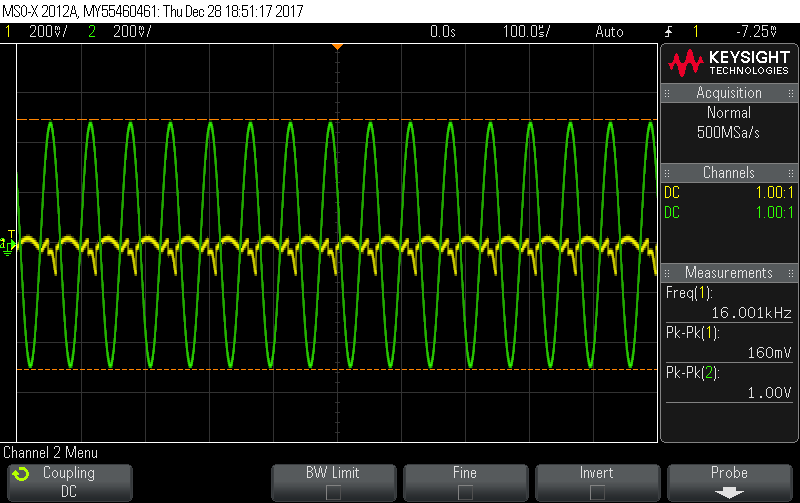
\includegraphics[width=0.45\unitlength]{lpf_osc2.png}
	\caption{\label{fig:lpfosc2}Practical Output Signal for 16 kHz}
\end{figure} 

		
\section{General Diagram}

	General diagram of the project can be seen at \textit{Figure~\ref{fig:diagram}}.

\begin{figure}[h!]
\setlength{\unitlength}{\textwidth}
\center 
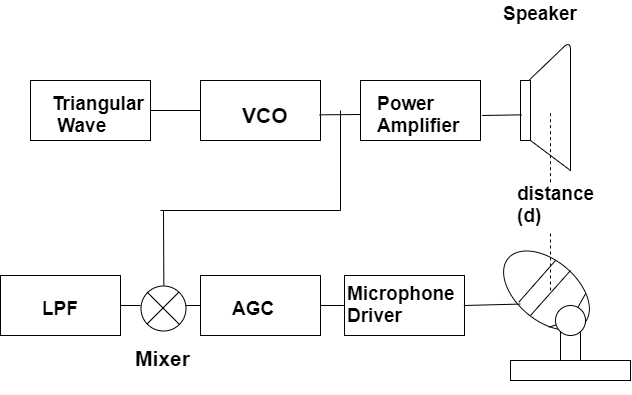
\includegraphics[width=0.5\unitlength]{diagram3.png}
\caption{\label{fig:diagram}General Diagram of the Project }
\end{figure}	

\vfill
\-\\[2cm]
		
\section{Overall Project}


	Overall project built at the laboratory can be seen at \textit{Figure~\ref{fig:overall}}.

\begin{figure*}[h!]
\setlength{\unitlength}{\textwidth}
\center 
\includegraphics[width=1.0\unitlength]{overall_cct2.jpg}
\caption{\label{fig:overall}Overall Project }
\end{figure*}	




\section{Conclusion}

	First, a triangular voltage is generated with varying frequencies by a VCO circuit and 10 Hz triangular wave input. Then modulated triangular wave is sent to microphone by a speaker and to mixer at the same time. The microphone transmits the captured signal to the mixer. In the mixer, there are two equivalent inputs but with a phase shift. Output of the mixer is basically sum of two waves having frequencies $ (f_1+f_2)$ and $(|~f_1 -f_2~|) $ that are frequencies of two inputs of the mixer. If this signal is low-passed, the filtered signal have $(|~f_1 -f_2~|) $ frequency. By measuring $(|~f_1 -f_2~|) $, the distance between the speaker and the microphone can be found by a simple algebra, $K*(|~f_1 -f_2~|) $ where K is a constant to be determined and having unit of $\frac{Meter}{Hertz} $.

 


\begin{thebibliography}{00}
\bibitem{b1} J.-J. Lin, Y.-P. Li, W.-C. Hsu, and T.-S. Lee, “Design of an FMCW radar baseband signal processing system for automotive application,” SpringerPlus, vol. 5, no. 1, 2016.	
\bibitem{b2} “LF353 Datasheet.” [Online]. Available: http://www.ti.com/lit/ds/symlink/lf353-n.pdf. [Accessed: 20-Jan-2018].
\bibitem{b3} “2N7000 Datasheet.” [Online]. Available: https://www.onsemi.com/pub/Collateral/2N7000-D.PDF. [Accessed: 20-Jan-2018].
\bibitem{b4} “LF353 Datasheet.” [Online]. Available: http://www.falstad.com/circuit/e-vco.html.

%\bibitem{b6} Y. Yorozu, M. Hirano, K. Oka, and Y. Tagawa, ``Electron spectroscopy studies on magneto-optical media and plastic substrate interface,'' IEEE Transl. J. Magn. Japan, vol. 2, pp. 740--741, August 1987 [Digests 9th Annual Conf. Magnetics Japan, p. 301, 1982].
%\bibitem{b7} M. Young, The Technical Writer's Handbook. Mill Valley, CA: University Science, 1989.
\end{thebibliography}

\end{document}